\pdfminorversion=4
\documentclass[aspectratio=169]{beamer}

\mode<presentation>
{
  \usetheme{default}
  \usecolortheme{default}
  \usefonttheme{default}
  \setbeamertemplate{navigation symbols}{}
  \setbeamertemplate{caption}[numbered]
  \setbeamertemplate{footline}[frame number]  % or "page number"
  \setbeamercolor{frametitle}{fg=white}
  \setbeamercolor{footline}{fg=black}
}

\usepackage[english]{babel}
\usepackage{inputenc}
\usepackage{tikz}
\usepackage{courier}
\usepackage{array}
\usepackage{bold-extra}
\usepackage{minted}
\usepackage[thicklines]{cancel}
\usepackage{fancyvrb}
\usepackage[normalem]{ulem}

\xdefinecolor{dianablue}{rgb}{0.18,0.24,0.31}
\xdefinecolor{darkblue}{rgb}{0.1,0.1,0.7}
\xdefinecolor{darkgreen}{rgb}{0,0.5,0}
\xdefinecolor{darkgrey}{rgb}{0.35,0.35,0.35}
\xdefinecolor{darkorange}{rgb}{0.8,0.5,0}
\xdefinecolor{darkred}{rgb}{0.7,0,0}
\definecolor{darkgreen}{rgb}{0,0.6,0}
\definecolor{mauve}{rgb}{0.58,0,0.82}

\title[2024-07-08-scipy-teen-track-talk-06]{What is a neural network?}
\author{Jim Pivarski}
\institute{Princeton University -- IRIS-HEP}
\date{July 8, 2024}

\usetikzlibrary{shapes.callouts}

\begin{document}

\logo{\pgfputat{\pgfxy(0.11, 7.4)}{\pgfbox[right,base]{\tikz{\filldraw[fill=dianablue, draw=none] (0 cm, 0 cm) rectangle (50 cm, 1 cm);}\mbox{\hspace{-8 cm}\includegraphics[height=1 cm]{princeton-logo-long.png}\hspace{0.1 cm}\raisebox{0.1 cm}{\includegraphics[height=0.8 cm]{iris-hep-logo-long.png}}\hspace{0.1 cm}}}}}

\begin{frame}
  \titlepage
\end{frame}

\logo{\pgfputat{\pgfxy(0.11, 7.4)}{\pgfbox[right,base]{\tikz{\filldraw[fill=dianablue, draw=none] (0 cm, 0 cm) rectangle (50 cm, 1 cm);}\mbox{\hspace{-8 cm}\includegraphics[height=1 cm]{princeton-logo.png}\hspace{0.1 cm}\raisebox{0.1 cm}{\includegraphics[height=0.8 cm]{iris-hep-logo.png}}\hspace{0.1 cm}}}}}

% Uncomment these lines for an automatically generated outline.
%\begin{frame}{Outline}
%  \tableofcontents
%\end{frame}

% START START START START START START START START START START START START START

\begin{frame}{\only<1>{Equation of a line (fitting $a$ and $b$ to measurements $y$ versus $x$)}\only<2>{Equation of a plane (height $y$ versus 2D coordinates $x_1$ and $x_2$)}\only<3>{Equation of a hyperplane (N-dimensional)}\only<4>{General linear transformation: many inputs, many outputs}\only<5>{Pass through function $f$ to make it non-linear}}
\vspace{0.25 cm}
\begin{onlyenv}<1>
\begin{center}
\includegraphics[width=0.4\linewidth]{equation-for-a-line.pdf}
\end{center}
\vspace{-1.5 cm}
\end{onlyenv}\begin{onlyenv}<2>
\begin{center}
\includegraphics[width=0.4\linewidth]{equation-for-a-plane.pdf}
\end{center}
\vspace{-1.75 cm}
\end{onlyenv}

\begin{columns}
\column{1.1\linewidth}
\renewcommand{\arraystretch}{1.5}
\scriptsize
\[ \uncover<5->{f \left[} \mbox{\hspace{0.25 cm}} \underbrace{\uncover<2->{\left(} \begin{array}{c c c c}
\only<2->{\uncover<4->{a_{1,1}} & \uncover<4->{a_{1,2}} & \uncover<4->{\ldots} & \uncover<4->{a_{1,10}} \\}
\only<2->{\uncover<4->{a_{2,1}} & \uncover<4->{a_{2,2}} & \uncover<4->{\ldots} & \uncover<4->{a_{2,10}} \\}
\only<2->{\only<2-3>{a_1}\only<4->{a_{3,1}} & \only<2-3>{a_2}\only<4->{a_{3,2}} & \uncover<3->{\ldots} & \uncover<3->{\only<1-3>{a_{10}}}\only<4->{a_{3,10}} \\}
\only<2->{\uncover<4->{a_{4,1}} & \uncover<4->{a_{4,2}} & \uncover<4->{\ldots} & \uncover<4->{a_{4,10}} \\}
\only<2->{\uncover<4->{a_{5,1}} & \uncover<4->{a_{5,2}} & \uncover<4->{\ldots} & \uncover<4->{a_{5,10}} \\}
\end{array}\only<1>{\mbox{\hspace{0.5 cm}}a\mbox{\hspace{0.5 cm}}} \vphantom{\vbox to 1.5cm{}} \uncover<2->{\right)}}_{\text{free parameters in the fit}} \cdot \underbrace{\uncover<2->{\left(} \only<1>{x}\begin{array}{c}
\only<2->{\uncover<2->{x_1} \\}
\only<2->{\uncover<2->{x_2} \\}
\only<2->{\uncover<3->{\vdots} \\}
\only<2->{\uncover<3->{x_{10}} \\}
\end{array} \vphantom{\vbox to 1.5cm{}} \uncover<2->{\right)}}_{\text{input values}} + \underbrace{\uncover<4->{\left(} \begin{array}{c}
\uncover<4->{b_1} \\
\uncover<4->{b_2} \\
\only<1-3>{b}\only<4->{b_3} \\
\uncover<4->{b_4} \\
\uncover<4->{b_5} \\
\end{array} \vphantom{\vbox to 1.5cm{}} \uncover<4->{\right)}}_{\text{free parameters}} \mbox{\hspace{0.25 cm}} \uncover<5->{\right]} = \underbrace{\uncover<4->{\left(} \begin{array}{c}
\uncover<4->{y_1} \\
\uncover<4->{y_2} \\
\only<1-3>{y}\only<4->{y_3} \\
\uncover<4->{y_4} \\
\uncover<4->{y_5} \\
\end{array} \vphantom{\vbox to 1.5cm{}} \uncover<4->{\right)}}_{\text{output values}} = \begin{array}{c}
\uncover<5->{f[} \uncover<4->{a_{1,1}x_1 + a_{1,2}x_2 + \ldots a_{1,10}x_{10} + b_1} \uncover<5->{]} \\
\uncover<5->{f[} \uncover<4->{a_{2,1}x_1 + a_{2,2}x_2 + \ldots a_{2,10}x_{10} + b_2} \uncover<5->{]} \\
\uncover<5->{f[} \only<1>{ax + b}\only<2-3>{a_{1}x_1 + a_{2}x_2 \uncover<3->{+ \ldots a_{10}x_{10}} + b}\only<4->{a_{3,1}x_1 + a_{3,2}x_2 + \ldots a_{3,10}x_{10} + b_3} \uncover<5->{]} \\
\uncover<5->{f[} \uncover<4->{a_{4,1}x_1 + a_{4,2}x_2 + \ldots a_{4,10}x_{10} + b_4} \uncover<5->{]} \\
\uncover<5->{f[} \uncover<4->{a_{5,1}x_1 + a_{5,2}x_2 + \ldots a_{5,10}x_{10} + b_5} \uncover<5->{]} \\
\end{array} \]
\end{columns}
\end{frame}

\begin{frame}{The non-linear function $f$ is called an ``activation function''}
\small
\vspace{0.5cm}
\begin{columns}
\column{0.2\linewidth}
\includegraphics[width=\linewidth]{Activation_binary_step.pdf}

\column{0.25\linewidth}
binary step

\vspace{-\baselineskip}
\[ f(x) = \left\{ \begin{array}{c l}
0 & \text{if } x < 0 \\
1 & \text{if } x \ge 0 \\
\end{array} \right. \]

\column{0.2\linewidth}
\includegraphics[width=\linewidth]{Activation_rectified_linear.pdf}

\column{0.3\linewidth}
rectified linear unit (ReLU)

\vspace{-\baselineskip}
\[ f(x) = \left\{ \begin{array}{c l}
0 & \text{if } x < 0 \\
x & \text{if } x \ge 0 \\
\end{array} \right. \]
\end{columns}

\vspace{0.5cm}
\begin{columns}
\column{0.2\linewidth}
\includegraphics[width=\linewidth]{Activation_logistic.pdf}

\column{0.25\linewidth}
logistic (soft step)

\vspace{-\baselineskip}
\[ f(x) = \frac{1}{1 + e^{-x}} \]

\column{0.2\linewidth}
\includegraphics[width=\linewidth]{Activation_prelu.pdf}


\column{0.3\linewidth}
``leaky'' ReLU

\vspace{-\baselineskip}
\[ f(x) = \left\{ \begin{array}{c l}
\alpha x & \text{if } x < 0 \\
x & \text{if } x \ge 0 \\
\end{array} \right. \]
\end{columns}

\vspace{0.5cm}
\begin{columns}
\column{0.2\linewidth}
\includegraphics[width=\linewidth]{Activation_tanh.pdf}

\column{0.25\linewidth}
hyperbolic tangent

\vspace{-\baselineskip}
\[ f(x) = \frac{e^x - e^{-x}}{e^x + e^{-x}} \]

\column{0.2\linewidth}
\includegraphics[width=\linewidth]{Activation_swish.pdf}

\column{0.3\linewidth}
sigmoid linear unit (``swish'')

\[ f(x) = \frac{x}{1 + e^{-x}} \]
\end{columns}

\large

\vspace{0.75 cm}
There are many choices, but ReLU is the simplest and most common.
\end{frame}

\begin{frame}{Neural networks take inspiration from neurons in the brain}
\begin{center}
\includegraphics[width=0.9\linewidth]{real-neuron.pdf}
\end{center}

\vspace{-1cm}
\begin{columns}
\column{1.1\linewidth}
\renewcommand{\arraystretch}{1.5}
\scriptsize
\[ f \left[ \mbox{\hspace{0.25 cm}} \underbrace{\left( \begin{array}{c c c c}
a_{1,1} & a_{1,2} & \ldots & a_{1,10} \\
a_{2,1} & a_{2,2} & \ldots & a_{2,10} \\
a_{3,1} & a_{3,2} & \ldots & a_{3,10} \\
a_{4,1} & a_{4,2} & \ldots & a_{4,10} \\
a_{5,1} & a_{5,2} & \ldots & a_{5,10} \\
\end{array} \vphantom{\vbox to 1.5cm{}} \right)}_{\text{free parameters in the fit}} \cdot \underbrace{\left( \begin{array}{c}
x_1 \\
x_2 \\
\vdots \\
x_{10} \\
\end{array} \vphantom{\vbox to 1.5cm{}} \right)}_{\text{input values}} + \underbrace{\left( \begin{array}{c}
b_1 \\
b_2 \\
b_3 \\
b_4 \\
b_5 \\
\end{array} \vphantom{\vbox to 1.5cm{}} \right)}_{\text{free parameters}} \mbox{\hspace{0.25 cm}} \right] = \underbrace{\left( \begin{array}{c}
y_1 \\
y_2 \\
y_3 \\
y_4 \\
y_5 \\
\end{array} \vphantom{\vbox to 1.5cm{}} \right)}_{\text{output values}} = \begin{array}{c}
f[ a_{1,1}x_1 + a_{1,2}x_2 + \ldots a_{1,10}x_{10} + b_1 ] \\
f[ a_{2,1}x_1 + a_{2,2}x_2 + \ldots a_{2,10}x_{10} + b_2 ] \\
f[ a_{3,1}x_1 + a_{3,2}x_2 + \ldots a_{3,10}x_{10} + b_3 ] \\
f[ a_{4,1}x_1 + a_{4,2}x_2 + \ldots a_{4,10}x_{10} + b_4 ] \\
f[ a_{5,1}x_1 + a_{5,2}x_2 + \ldots a_{5,10}x_{10} + b_5 ] \\
\end{array} \]
\end{columns}
\end{frame}

\begin{frame}{Neural networks take inspiration from neurons in the brain}
\vspace{0.15 cm}
\begin{columns}
\column{1.2\linewidth}
\includegraphics[width=\linewidth]{nerve-cells-sem-steve-gschmeissner.jpg}
\end{columns}
\end{frame}

\begin{frame}{Neural networks take inspiration from neurons in the brain}
\vspace{0.16 cm}
\begin{columns}
\column{1.1\linewidth}
\includegraphics[width=\linewidth]{real-neuron-layers.pdf}
\end{columns}
\end{frame}

\begin{frame}{Neural networks take inspiration from neurons in the brain}
To do the same thing with our model, take the output of one ``activation + linear transform'' and use it as the input to the next:

\vspace{1 cm}\only<4>{\vspace{-0.5 cm}}
\begin{columns}
\column{1.15\linewidth}
\[ \only<1>{f \left( a^{\text{layer 1}}_{i\mbox{,\,}j} \cdot x_j + b^{\text{layer 1}}_i \right)}\only<2>{f \left( a^{\text{layer 2}}_{i\mbox{,\,}j} \cdot \fbox{$\displaystyle f \left( a^{\text{layer 1}}_{i\mbox{,\,}j} \cdot x_j + b^{\text{layer 1}}_i \right)$} + b^{\text{layer 2}}_i \right)}\only<3>{f \left( a^{\text{layer 3}}_{i\mbox{,\,}j} \cdot \fbox{$\displaystyle f \left( a^{\text{layer 2}}_{i\mbox{,\,}j} \cdot \fbox{$\displaystyle f \left( a^{\text{layer 1}}_{i\mbox{,\,}j} \cdot x_j + b^{\text{layer 1}}_i \right)$} + b^{\text{layer 2}}_i \right) $} + b^{\text{layer 3}}_i \right)}\only<4>{f \left( a^{\text{layer 4}}_{i\mbox{,\,}j} \cdot \fbox{$\displaystyle f \left( a^{\text{layer 3}}_{i\mbox{,\,}j} \cdot \fbox{$\displaystyle f \left( a^{\text{layer 2}}_{i\mbox{,\,}j} \cdot \fbox{$\displaystyle f \left( a^{\text{layer 1}}_{i\mbox{,\,}j} \cdot x_j + b^{\text{layer 1}}_i \right)$} + b^{\text{layer 2}}_i \right) $} + b^{\text{layer 3}}_i \right) $} + b^{\text{layer 4}}_i \right)} \]
\end{columns}
\end{frame}

\begin{frame}{It's usually drawn like this}
\vspace{0.25 cm}
\only<1>{\includegraphics[width=\linewidth]{artificial-neural-network-layers.pdf}}\only<2>{\includegraphics[width=\linewidth]{artificial-neural-network-layers-2.pdf}}

\vspace{0.25 cm}
The lines indicate that every output from one layer is included in the linear transformation of the next layer. (``There's an $a_{i\mbox{,\,}j}$ for every $x_j$ and $y_i$.'')
\end{frame}

\begin{frame}{Connectivism: automatic learning by fitting the $a_{i\mbox{,\,}j}$, $b_i$ parameters}
\small
\vspace{0.2 cm}
\begin{columns}
\column{0.4\linewidth}
\includegraphics[width=\linewidth]{330-PSA-80-60_\(USN_710739\)_\(20897323365\).jpg}

Frank Rosenblatt's perceptron machine (1958) attempted to recognize images of letters.

\vspace{0.2 cm}
\begin{minipage}{1.1\linewidth}\raggedright
The free parameters were adjusted with motors. This system eventually learned left-versus-right (not much more).
\end{minipage}

\column{0.6\linewidth}
\includegraphics[width=\linewidth]{Organization_of_a_biological_brain_and_a_perceptron.png}
\end{columns}
\end{frame}

\begin{frame}{More inspiration from nature: eye-neurons are not fully connected}
\vspace{0.35 cm}
\begin{center}
\includegraphics[width=0.5\linewidth]{eye-neurons.jpg}
\end{center}

\vspace{0.25 cm}
Neurons in one layer are connected to only a few of the neurons in the next layer.
\end{frame}

\begin{frame}{``Convolutional'' (restricted) neural network}
\vspace{0.25 cm}
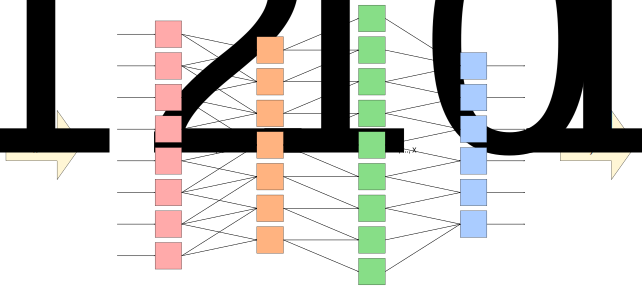
\includegraphics[width=\linewidth]{convolutional-neural-network-layers.pdf}

\vspace{0.25 cm}
This sets a lot of $a_{i\mbox{,\,}j}$ parameters to zero and doesn't let them be tuned in the fit.
\end{frame}

\begin{frame}{Kunihiko Fukushima's neocognitron (1980)}
\vspace{0.15 cm}
\begin{center}
\includegraphics[width=0.75\linewidth]{higher-order-features.png}
\end{center}

\vspace{0.15 cm}
\begin{columns}
\column{0.45\linewidth}
\includegraphics[width=\linewidth]{convolutional-planes.png}

\column{0.45\linewidth}
\includegraphics[width=\linewidth]{convolutional-recognition.png}
\end{columns}
\end{frame}

\begin{frame}{Each layer of a neural network is more abstract than the last}
\vspace{0.25 cm}
\includegraphics[width=\linewidth]{convolutional-neural-network-layers-labeled.pdf}
\end{frame}

\begin{frame}{Fun fact: mice have hawk-shaped features in their visual networks}
\small
\vspace{0.5 cm}
\begin{columns}
\column{0.35\linewidth}
\includegraphics[width=\linewidth]{mouse.png}

\column{0.35\linewidth}
\includegraphics[width=\linewidth]{hawk-shaped-features.jpg}
\end{columns}

\vspace{0.75 cm}
Y.\ Zhang, I.\ Kim, J.\ Sanes, {\it The most numerous ganglion cell type of the mouse retina is a selective feature detector} (2012), \textcolor{blue}{\url{https://doi.org/10.1073/pnas.1211547109}}
\end{frame}

\begin{frame}{These ideas have been studied for a long time}
\vspace{0.2 cm}
\begin{columns}
\column{1.1\linewidth}
\only<1>{\includegraphics[width=\linewidth]{ups-and-downs-of-ai.png}}\only<2>{\includegraphics[width=\linewidth]{ups-and-downs-of-ai-overlay.png}}
\end{columns}
\end{frame}

\begin{frame}{Why are neural networks only a big thing now?}
\vspace{0.5 cm}
\begin{enumerate}\setlength{\itemsep}{0.5 cm}
\item<1-> At first, neural networks were much worse than ``symbolic'' (rule-based) approaches. Learning without explicit rules seemed like magical thinking or hype.

\item<2-> Important algorithmic discoveries: gradient descent, backpropagation, ReLU activation, convolutional and recurrent topologies, Xavier initialization, transfer learning, batch normalization, dropout, the attention mechanism, \ldots

\item<3-> Large enough datasets, already digitized, to expose all the nuances of human-like behaviors: the world wide web.

\item<4-> Large enough compute farms and GPUs to analyze the above.
\end{enumerate}
\end{frame}

\end{document}
